\documentclass[portrait,paperwidth=24in,paperheight=36in,fontscale=0.4]{baposter} %,a0paper
\newif\ifisneurips
\isneuripsfalse

\tracingstats=2

\usepackage{epstopdf}
\usepackage{graphicx}
\usepackage{amsmath}
\usepackage{amssymb}
\usepackage{relsize}
\usepackage{multirow}
\usepackage{bm}
\usepackage{booktabs}
\usepackage{colortbl}
\usepackage{algorithm}
\usepackage{algorithmic}
\usepackage{cancel}

\usepackage{graphicx}
\usepackage{multicol}


\usepackage{times}
\usepackage{helvet}
%\usepackage{bookman}
\usepackage{palatino}
%\usepackage[outdir=./]{epstopdf}

\newcommand{\captionfont}{\footnotesize}

\selectcolormodel{cmyk}
\let\polishl\l

%%%%%%%%%%%%%%%%%%%%%%%%%%%%%%%%%%%%%%%%%%%%%%%%%%%%%%%%%%%%%%%%%%%%%%%%%%%%%%%%
%%%% Math symbols used in the text. Shared with paper
%%%%%%%%%%%%%%%%%%%%%%%%%%%%%%%%%%%%%%%%%%%%%%%%%%%%%%%%%%%%%%%%%%%%%%%%%%%%%%%%
\def\opt{{\textsc{OPT}_k}}
\def\const{{\mathrm{const}}}
\def\nnz{{\mathrm{nnz}}}
\def\r{\sfrac{\sigma_{\w}^2}{\sigma_{\xib}^2}}
\def\rm{\sfrac{\sigma_{\xib}^2}{\sigma_{\w}^2}}
\def\cmark{\Green{\checkmark}}
\def\xmark{\Red{\large\sffamily x}}
\newcommand{\pdet}{{\mathrm{pdet}}}
\newcommand{\MSPE}[1] {{\mathrm{MSPE}\big[#1\big]}}
\newcommand{\MSE}[1] {{\mathrm{MSE}\big[#1\big]}}
\def\Poisson{{\operatorname{Poisson}}}
\def\PB{{\operatorname{PB}}}
\newcommand{\DP}[1]{\mathcal{DP}^{#1}}
\def\Ic{\mathcal{I}}
\def\Jc{\mathcal{J}}
\def\Mc{\mathcal M}
\def\Ec{\mathcal E}
\def\sr{{\mathrm{sr}}}
\def\ktd{{k^{\underline{d}}}}
\def\Det{{\mathrm{Det}}}
\def\detu{{\widecheck{\mathrm{Det}}_\mu^\gamma}}
\def\deto{{\widehat{\mathrm{Det}}_\mu^\gamma}}
\def\Zu{{\widecheck{Z}_\mu^{\gamma}}}
\def\Zo{{\widehat{Z}_\mu^{\gamma}}}
\def\Zun{{\widecheck{Z}_\mu^{\gamma_n}}}
\def\Zon{{\widehat{Z}_\mu^{\gamma_n}}}
\newcommand{\Er}{\mathrm{Er}}
\newif\ifDRAFT
\DRAFTtrue
\ifDRAFT
\newcommand{\marrow}{\marginpar[\hfill$\longrightarrow$]{$\longleftarrow$}}
\newcommand{\niceremark}[3]
   {\textcolor{red}{\textsc{#1 #2:} \marrow\textsf{#3}}}
\newcommand{\ken}[2][says]{\niceremark{Ken}{#1}{#2}}
\newcommand{\manfred}[2][says]{\niceremark{Manfred}{#1}{#2}}
\newcommand{\michael}[2][says]{\niceremark{Michael}{#1}{#2}}
\newcommand{\michal}[2][says]{\niceremark{Michal}{#1}{#2}}
\newcommand{\feynman}[2][says]{\niceremark{Feynman}{#1}{#2}}
%\usepackage[inline]{showlabels}
\else
\newcommand{\ken}[1]{}
\newcommand{\michael}[1]{}
\newcommand{\michal}[1]{}
\newcommand{\feynman}[1]{}
\fi
\newcommand{\norm}[1]{{\| #1 \|}}

\newcommand{\deff}{d_{\textnormal{eff}}}
\def\ee{\mathrm{e}}
\newcommand\mydots{\makebox[1em][c]{.\hfil.\hfil.}}
\def\Sd{\mathscr{S}_{\!d}}
\newcommand{\dx}{\dxy_{\!\cal X}}
\newcommand{\dxk}{\dxy_{\!\cal X}^k}
\newcommand{\dk}{\dxy^k}
\newcommand{\dxy}{\mathrm{D}}
\def\simiid{\overset{\textnormal{\fontsize{6}{6}\selectfont
i.i.d.}}{\sim}}
%\newcommand{\Dxy}{D_{\!\cal X\!,\cal Y}}
\def\vskx{{\mathrm{VS}_{\!\dx}^k}}
\def\vsk{{\mathrm{VS}_{\!D}^k}}
\def\vskxm{{\mathrm{VS}_{\!\dx}^{k-1}}}
\def\vskm{{\mathrm{VS}_{\!D}^{k-1}}}
\def\vsdx{{\mathrm{VS}_{\!\dx}^d}}
\def\vsd{{\mathrm{VS}_{\!D}^d}}
\newcommand{\vs}[1]{{\mathrm{VS}_{\!D}^{#1}}}
\newcommand{\sigd}{\boldsymbol\Sigma_{\!\dx}}
\def\wols{\w_{\mathrm{LS}}}
\def\wds{\boldsymbol\w_{\!D}^*}
\def\kd{K_{\!\dx}}

\def\poly{{\mathrm{poly}}}
\def\polylog{{\mathrm{polylog}}}
\def\DPP{{\mathrm{DPP}}}
\def\DPPcor{{\DPP_{\!\mathrm{cor}}}}
\def\DPPens{{\DPP_{\!\mathrm{ens}}}}
\newcommand{\DPPreg}[1]{{\DPP_{\!\mathrm{reg}}^{#1}}}
\def\Vol{{\mathrm{VS}}}
\def\Lev{{\mathrm{Lev}}}
\newcommand\todod[1]{\Red{\# DH: #1}}
\newcommand{\explain}[2]{\mathrel{\overset{\makebox[0pt]{\text{\tiny
#1}}}{#2}}}
\def\tot {{\mathrm{tot}}}
\def\checkmark{\tikz\fill[scale=0.4](0,.35) -- (.25,0) --
(1,.7) -- (.25,.15) -- cycle;}
\newcommand{\mnote}[1]{{\bf\large \Magenta{*}}\marginpar{\small \Magenta{#1}}}
\newcommand{\bnote}[1]{{\bf #1}}

\newcommand{\sqrtshort}[1]{{\sqrt{\white{\Big|}\!\!\smash{\text{\fontsize{9}{9}\selectfont$#1$}}}}}
\newenvironment{proofof}[2]{\par\vspace{2mm}\noindent\textbf{Proof of {#1} {#2}}\ }{\hfill\BlackBox}
\newcommand{\sets}[2]
{{\hspace{-0.3mm}[\hspace{-0.3mm}#1\hspace{-0.3mm}]\hspace{-0.3mm}\choose
\hspace{-0.3mm}#2\hspace{-0.3mm}}}
\DeclareMathOperator{\sgn}{\textnormal{sgn}}
\DeclareMathOperator{\adj}{\textnormal{adj}}
\def\Rb{{\mathbf{R}}}
\DeclareMathOperator{\ws}{\widetilde{\w}}
\newcommand{\inote}[1]{{\bf {#1}}}
\def\xib{\boldsymbol\xi}
\def\Sigmab{\mathbf{\Sigma}}
\def\Sigmabh{\widehat{\Sigmab}}
\def\Sigmabt{\widetilde{\Sigmab}}
\def\S{\mathbf{S}}
\def\T{\mathbf{T}}
\def\xt{\tilde{x}}
\def\xbt{\widetilde{\x}}
\def\xbh{\widehat{\x}}
\def\ubh{\widehat{\u}}
\def\dom {{\mathrm{dom}}}
\def\val {{\mathrm{val}}}
\def\out {{\mathrm{out}}}
\def\iin  {{\mathrm{iin}}}
\def\s {\mathbf{s}}
\def\q {\mathbf{q}}
\def\qt{\tilde{q}}
\def\itld {j}
\def\ubt {\tilde{\u}}
\def\n{\{1..n\}}
\def\cb {\mathbf{c}}
\def\cW{\mathcal W}
\def\Xt{\widetilde{X}}
\def\Dbt{\widetilde{\D}}
\def\xtb{\tilde{\mathbf{x}}}
\def\ytb{\tilde{\mathbf{y}}}
\def\Xtb{\widetilde{\mathbf{X}}}
\def\Xbb{\overline{\X}}
\def\Xb{{\bar{\X}}}
\def\ybb{\overline{\y}}
\def\f{{\mathbf{f}}}
\def\g{{\mathbf{g}}}
\def\fbb{{\overline{\f}}}
\def\fb{{\overline{f}}}
\def\Xc{\mathcal{X}}
\def\W{\mathbf W}
\def\L{\mathbf{L}}
\def\Rb{\mathbf R}
\def\Pc{\mathcal{P}}
\def\Nc{\mathcal{N}}
\def\Pt{\widetilde{P}}
\def\Hc{\mathcal{H}}
\def\Wc{\mathcal{W}}
\def\Cc{\mathcal{C}}
\def\p{\mathbf p}
%\def\r{\mathbf r}
\def\Y{\mathbf Y}
\def\H{\mathbf H}
\def\K{\mathbf K}
\def\Kh{\widehat{K}}
\def\Kbh{{\widehat{\K}}}
\def\Q{\mathbf Q}
\def\Qbar{{\bar{\mathbf Q}}}
\def\Ytb{\widetilde{\mathbf{Y}}}
\def\c{{n-d\choose s-d}}
\DeclareMathOperator{\Proj}{Proj}
\newcommand{\Span}{\mathrm{span}}
\newcommand{\ofsubt}[1]{\mbox{\scriptsize \raisebox{0.25pt}{$(#1)$}}}
%\raisebox{0.5pt}{$($}}#1\mbox{\tiny \raisebox{0.5pt}{$)$}}}
\newcommand{\ofsub}[1]{\mbox{\small \raisebox{0.0pt}{$(#1)$}}}
%\newcommand{\ofsubb}[1]{\mbox{\footnotesize \raisebox{0.5pt}{$(#1)$}}}
%\newcommand{\ofsub}[1]{(#1)}
%\newcommand{\ofsub}[1]{\mbox{\tiny$|$\hspace{-0.5pt}\raisebox{-0.5pt}{$#1$}}}
\newcommand{\of}[2]{{#1{\!\ofsub{#2}}}}
\newcommand{\oft}[2]{{#1{\!\ofsubt{#2}}}}
\newcommand{\fof}[2]{{#1({#2})}}
\newcommand{\yof}[2]{{#1{\ofsub{#2}}}}
%\newcommand{\yofb}[2]{{#1{\ofsubb{#2}}}}
\newcommand{\lazy}{FastRegVol}
\newcommand{\volsamp}{RegVol}

\newcommand{\Sm}{{S_{-i}}}
\newcommand{\Sp}{{S_{+i}}}
\ifx\BlackBox\undefined
\newcommand{\BlackBox}{\rule{1.5ex}{1.5ex}}  % end of proof
\fi
%\renewcommand{\dagger}{+}
\DeclareMathOperator*{\argmin}{\mathop{\mathrm{argmin}}}
\DeclareMathOperator*{\argmax}{\mathop{\mathrm{argmax}}}
\DeclareMathOperator*{\diag}{\mathop{\mathrm{diag}}}
\def\x{\mathbf x}
\def\y{\mathbf y}
\def\ybh{\widehat{\mathbf y}}
\def\ybb{\bar{\mathbf y}}
\def\xbb{\bar{\mathbf x}}
\def\yb{{\bar y}}
\def\ybt{\widetilde{\mathbf y}}
\def\yh{\widehat{y}}
\def\yhb{\widehat{\y}}
\def\yt{\widetilde{y}}
\def\z{\mathbf z}
\def\a{\mathbf a}
\def\b{\mathbf b}
\def\w{\mathbf w}
\def\v{\mathbf v}
\def\m{\mathbf m}
\def\wbh{\widehat{\mathbf w}}
\def\wh{\widehat{\mathbf w}}
\def\vbh{\widehat{\mathbf v}}
\def\wbt{\widetilde{\mathbf w}}
\def\e{\mathbf e}
\def\zero{\mathbf 0}
\def\one{\mathbf 1}
\def\u{\mathbf u}
\def\ubbar{\bar{\mathbf u}}
\def\f{\mathbf f}
\def\ellb{\boldsymbol\ell}

\def\X{\mathbf X}
\def\Xs{\widetilde{\X}}
\def\B{\mathbf B}
\def\A{\mathbf A}
\def\C{\mathbf C}
\def\U{\mathbf U}
\def\Ubt{\widetilde{\mathbf U}}
\def\Ubh{\widehat{\mathbf U}}
\def\Ubbar{\bar{\mathbf U}}
\def\F{\mathbf F}
\def\D{\mathbf D}
\def\V{\mathbf V}
\def\M{\mathbf M}
\def\Mh{\widehat{\mathbf M}}
%\def\S{\mathbf S}
\def\Stb{\widetilde{\mathbf{S}}}
\def\Sbh{\widehat{\mathbf{S}}}
\def\St{\widetilde{\S}}
\def\Sh{\widehat{S}}
\def\Sc{\mathcal{S}}
\def\Fc{\mathcal{F}}
\def\Vc{\mathcal{V}}
\def\Bc{\mathcal{B}}
\def\Dc{\mathcal{D}}
\def\Z{\mathbf Z}
\def\Zbh{\widehat{\mathbf Z}}
\def\Zbt{\widetilde{\mathbf Z}}
\def\Abh{\widehat{\mathbf A}}
\def\I{\mathbf I}
\def\Ic{\mathcal I}
\def\II{\mathbf {I \!\,I}}
%\def\II{\boldsymbol {\mathbb I}}
\def\A{\mathbf A}
\def\P{\mathbf P}
\def\Ph{\widehat{\mathbf P}}
\def\cP{\mathcal P}
\def\cR{\mathcal R}
\def\Xt{\widetilde{\mathbf{X}}}
\def\Xh{\widehat{\mathbf{X}}}
\def\Rh{\widehat{R}}
\def\Ot{\widetilde{O}}
\def\At{\widetilde{\A}}


\def\E{\mathbb E}
\def\R{\mathbb R}
\def\N{\mathbb N}
\def\Pr{\mathrm{Pr}}
%\def\C{\mathbb C}
\def\tr{\mathrm{tr}}
\def\Sbar{{\bar{S}}}
\def\cS{{\mathcal{S}}}
\def\Tbar{{\bar{T}}}
\def\Tt{{\widetilde{T}}}
\def\rank{\mathrm{rank}}
\def\Prob{\mathrm{Prob}}
\def\Var{\mathrm{Var}}
\def\Xinv{(\X^\top\X)^{-1}}
\def\XinvS{(\X_S\X_S^\top)^{-1}}
\def\ABinvS{(\A_S\B_S^\top)^{-1}}
\def\ABinv{(\A\B^\top)^{-1}}
\def\xinv{\x_i^\top\Xinv\x_i}
\def\Xinvr{(\lambda\I+\X_{-1}^\top\X_{-1})^{-1}}
\def\pdet{\mathrm{pdet}}
\newcommand{\vol}{\mathrm{vol}}
%\newcommand{\defeq}{:=}
\newcommand{\defeq}{\stackrel{\textit{\tiny{def}}}{=}}
\newcommand{\di}{{[d+1]_{-i}}}
\newcommand{\cov}{\mathrm{cov}}
\let\origtop\top
\renewcommand\top{{\scriptscriptstyle{\origtop}}} % this makes transpose not so big

\definecolor{silver}{cmyk}{0,0,0,0.3}
\definecolor{yellow}{cmyk}{0,0,0.9,0.0}
\definecolor{reddishyellow}{cmyk}{0,0.22,1.0,0.0}
\definecolor{black}{cmyk}{0,0,0.0,1.0}
\definecolor{darkYellow}{cmyk}{0.2,0.4,1.0,0}
\definecolor{orange}{cmyk}{0.0,0.7,0.9,0}
\definecolor{darkSilver}{cmyk}{0,0,0,0.1}
\definecolor{grey}{cmyk}{0,0,0,0.5}
\definecolor{darkgreen}{cmyk}{0.6,0,0.8,0}
\newcommand{\Red}[1]{{\color{red}  {#1}}}
\newcommand{\Purple}[1]{{\color{purple}  {#1}}}
\newcommand{\Magenta}[1]{{\color{magenta}{#1}}}
\newcommand{\Green}[1]{{\color{darkgreen}  {#1}}}
\newcommand{\Blue}[1]{\color{blue}{#1}\color{black}}
\newcommand{\Orange}[1]{\textcolor{orange}{#1}\color{black}}
\newcommand{\Brown}[1]{{\color{brown}{#1}\color{black}}}
\newcommand{\Grey}[1]{{\color{grey}{#1}\color{black}}}
\newcommand{\white}[1]{{\textcolor{white}{#1}}}
\newcommand{\yellow}[1]{{\textcolor{reddishyellow}{#1}}}
\newcommand{\darkYellow}[1]{{\textcolor{darkYellow}{#1}}}
\newcommand{\grey}[1]{{\textcolor{grey}{#1}}}

\DeclareMathOperator{\half}{\frac{1}{2}}

\ifx\proof\undefined
\newenvironment{proof}{\par\noindent{\bf Proof\ }}{\hfill\BlackBox\\[2mm]}
\fi

\ifx\theorem\undefined
\newtheorem{theorem}{Theorem}
\fi

\ifx\example\undefined
\newtheorem{example}{Example}
\fi

\ifx\condition\undefined
\newtheorem{condition}{Condition}
\fi
\ifx\property\undefined
\newtheorem{property}{Property}
\fi

\ifx\lemma\undefined
\newtheorem{lemma}{Lemma}
\fi

\ifx\proposition\undefined
\newtheorem{proposition}{Proposition}
\fi

\ifx\remark\undefined
\newtheorem{remark}{Remark}
\fi

\ifx\corollary\undefined
\newtheorem{corollary}{Corollary}
\fi

\ifx\definition\undefined
\newtheorem{definition}{Definition}
\fi

\ifx\conjecture\undefined
\newtheorem{conjecture}{Conjecture}
\fi

\ifx\axiom\undefined
\newtheorem{axiom}{Axiom}
\fi

\ifx\claim\undefined
\newtheorem{claim}{Claim}
\fi

\ifx\assumption\undefined
\newtheorem{assumption}{Assumption}
\fi

\ifx\condition\undefined
\newtheorem{condition}{Condition}
\fi

\usepackage{tikz}
\usetikzlibrary{positioning}
%\usepgflibrary{shapes.symbols}
%\usetikzlibrary{shapes.geometric}

\newcommand{\bipgraph}[2]{%
    \begin{tikzpicture}[baseline=+.9 ex,rotate=90,scale=.18,every node/.style={circle,draw}]
    \foreach \xitem in {1,2,...,#1}
    {%
    % first set
    \node at (0,\xitem) (a\xitem) {};
    % second set
    \node at (2,\xitem) (b\xitem) {};   
    }%

    % connections
    \foreach \x [count=\xi] in {#2}
    {% 
    \foreach \tritem in \x % <-- Here no braces to make it a foreach list also not \xi but \x
    \draw(a\xi) -- (b\tritem);
    }
    \end{tikzpicture}  
}



%%%%%%%%%%%%%%%%%%%%%%%%%%%%%%%%%%%%%%%%%%%%%%%%%%%%%%%%%%%%%%%%%%%%%%%%%%%%%%%%
% Multicol Settings
%%%%%%%%%%%%%%%%%%%%%%%%%%%%%%%%%%%%%%%%%%%%%%%%%%%%%%%%%%%%%%%%%%%%%%%%%%%%%%%%
\setlength{\columnsep}{0.7em}
\setlength{\columnseprule}{0mm}
\setlength{\arrayrulewidth}{1pt} 


%%%%%%%%%%%%%%%%%%%%%%%%%%%%%%%%%%%%%%%%%%%%%%%%%%%%%%%%%%%%%%%%%%%%%%%%%%%%%%%%
% Save space in lists. Use this after the opening of the list
%%%%%%%%%%%%%%%%%%%%%%%%%%%%%%%%%%%%%%%%%%%%%%%%%%%%%%%%%%%%%%%%%%%%%%%%%%%%%%%%
\newcommand{\compresslist}{%
\setlength{\itemsep}{1pt}%
\setlength{\parskip}{0pt}%
\setlength{\parsep}{0pt}%
}


%%%%%%%%%%%%%%%%%%%%%%%%%%%%%%%%%%%%%%%%%%%%%%%%%%%%%%%%%%%%%%%%%%%%%%%%%%%%%%
%%% Begin of Document
%%%%%%%%%%%%%%%%%%%%%%%%%%%%%%%%%%%%%%%%%%%%%%%%%%%%%%%%%%%%%%%%%%%%%%%%%%%%%%

\begin{document}

%%%%%%%%%%%%%%%%%%%%%%%%%%%%%%%%%%%%%%%%%%%%%%%%%%%%%%%%%%%%%%%%%%%%%%%%%%%%%%
%%% Here starts the poster
%%%---------------------------------------------------------------------------
%%% Format it to your taste with the options
%%%%%%%%%%%%%%%%%%%%%%%%%%%%%%%%%%%%%%%%%%%%%%%%%%%%%%%%%%%%%%%%%%%%%%%%%%%%%%
% Define some colors
\definecolor{silver}{cmyk}{0,0,0,0.3}
\definecolor{yellow}{cmyk}{0,0,0.9,0.0}
\definecolor{reddishyellow}{cmyk}{0,0.22,1.0,0.0}
\definecolor{black}{cmyk}{0,0,0.0,1.0}
\definecolor{darkYellow}{cmyk}{0,0,1.0,0.5}
\definecolor{darkSilver}{cmyk}{0,0,0,0.1}


\definecolor{brightyellow}{cmyk}{0,0,0.7,0.0}
\definecolor{lightyellow}{cmyk}{0,0,0.3,0.0}
\definecolor{lighteryellow}{cmyk}{0,0,0.1,0.0}
\definecolor{lightestyellow}{cmyk}{0,0,0.05,0.0}

%%
\typeout{Poster Starts}
\background{}

\newlength{\leftimgwidth}
\begin{poster}%
  % Poster Options
  {
  % Show grid to help with alignment
  grid=false,
  % Column spacing
  colspacing=1em,
  % Color style
  bgColorOne=lighteryellow,
  bgColorTwo=lightestyellow,
  borderColor=reddishyellow,
  headerColorOne=yellow,
  headerColorTwo=reddishyellow,
  headerFontColor=black,
  boxColorOne=white,
  boxColorTwo=lighteryellow,
  % Format of textbox
  textborder=roundedleft,
%  textborder=rectangle,
  % Format of text header
  eyecatcher=true,
  headerborder=open,
  headerheight=0.09\textheight,
  headershape=roundedright,
  headershade=plain,
  headerfont=\Large\textsf, %Sans Serif
  boxshade=plain,
  background=shadeTB,
  linewidth=2pt
  }
  % Eye Catcher
  {} % No eye catcher for this poster. (eyecatcher=no above). If an eye catcher is present, the title is centered between eye-catcher and logo.
  % Title
  { \huge\sf
Minimax \ experimental \ design \\
\large Bridging  the  gap  between  statistical  and
 worst-case approaches  to
  least  squares  regression
    \vspace{.8em}}
  % Authors
{\sf
\begin{tabular}{c@{\qquad}c@{\qquad}c@{\qquad}c}
  Micha{\polishl} Derezi\'{n}ski
  & Kenneth L.~Clarkson
  & Michael W.~Mahoney
  & Manfred K.~Warmuth
  \\[1mm]

\includegraphics[height=1.5em]{../sty/Berkeley.png}
  &
\includegraphics[height=1.5em]{../sty/IBM.png}
  & 
\includegraphics[height=1.5em]{../sty/Berkeley.png}
  & 
\includegraphics[height=1.5em,viewport=0 160 375 261,clip]{../sty/UCSC}
      \hspace{1mm}
	
\includegraphics[height=1.5em] {../sty/Google.jpg}
\end{tabular}
\vspace{-1em} % bring logos down a bit so title does not touch top
}
% University logo
{}
\tikzstyle{light shaded}=[top color=baposterBGtwo!30!white,bottom color=baposterBGone!30!white,shading=axis,shading angle=30]


%%%%%%%%%%%%%%%%%%%%%%%%%%%%%%%%%%%%%%%%%%%%%%%%%%%%%%%%%%%%%%%%%%%%%%%%%%%%%%
%%% Now define the boxes that make up the poster
%%%---------------------------------------------------------------------------
%%% Each box has a name and can be placed absolutely or relatively.
%%% The only inconvenience is that you can only specify a relative position 
%%% towards an already declared box. So if you have a box attached to the 
%%% bottom, one to the top and a third one which should be in between, you 
%%% have to specify the top and bottom boxes before you specify the middle 
%%% box.
%%%%%%%%%%%%%%%%%%%%%%%%%%%%%%%%%%%%%%%%%%%%%%%%%%%%%%%%%%%%%%%%%%%%%%%%%%%%%%

\fboxsep=3pt
%\fboxsep=0mm%padding thickness
\fboxrule=1pt%border thickness

%%%%%%%%%%%%%%%%%%%%%%%%%%%%%%%%%%%%%%%%%%%%%%%%%%%%%%%%%%%%%%%%%%%%%%%%%%%%%%
\headerbox{Classical experimental design}{name=related,column=0,row=0,
  boxColorOne=white}{
  Consider $n$ vectors:
  $\x_1,\dots,\x_n\in\R^d$.\\
  Each $\x_i$ has a hidden random response $y_i$:
  \begin{align*}
    y_i = \x_i^\top\w^* + \xi_i,\qquad \xi_i\sim\Nc(0,\sigma^2)
  \end{align*}
  
\textbf{Task:} Select $k\ll n$ responses to query\\
  
\begin{minipage}[L]{0.4\textwidth}
\vspace{0.8cm}
Select $S=\{4,6,9\}$\\
\vspace{1cm}
Receive $y_4, y_6, y_9$
\end{minipage}
\begin{minipage}[R]{0.5\textwidth}
\begin{center}
	\begin{tikzpicture}[scale=0.9]
          \draw [fill=brown!30] (-2,0) rectangle (0,3);
          \draw [color=black] (-2,2) -- (0,2);
          \draw (-2.25,2) node {\mbox{\footnotesize $\x_4^\top$}}; 
          \draw [color=black] (-2,1.5) -- (0,1.5);
          \draw (-2.25,1.5) node {\mbox{\footnotesize $\x_6^\top$}}; 
          \draw [color=black] (-2,0.5) -- (0,0.5);
          \draw (-2.25,0.5) node {\mbox{\footnotesize $\x_9^\top$}}; 
	   \draw (-2.5,3) node {$\X$}; 
           \draw [decorate,decoration={brace}] (-2,3.1) -- (0,3.1);
          \draw (-1,3.4) node {\mbox{\fontsize{8}{8}\selectfont $d$}}; 
            \draw [color=lightgray,line width =0.5mm] (1,0) -- (1,3);
            \draw [color=lightgray] (0.75,3) node {$\y$};
            \draw (0.75,2) node {\mbox{\footnotesize $y_4$}}; 
            \draw (1,2) node {.}; 
            \draw[mark=*,mark size=1.5pt] plot coordinates{(1,2)};
            \draw (0.75,1.5) node {\mbox{\footnotesize $y_6$}}; 
            \draw (1,1.5) node {.}; 
            \draw[mark=*,mark size=1.5pt] plot coordinates{(1,1.5)};
            \draw (0.75,0.5) node {\mbox{\footnotesize $y_9$}}; 
            \draw[mark=*,mark size=1.5pt] plot coordinates{(1,.5)};
	\end{tikzpicture}
\end{center}
\end{minipage}
\vspace{5mm}

\textbf{Goal:}
Find the \emph{best unbiased estimator }of $\w^*$
\vspace{2mm}
%%%%%%%%%%%%%%%%%%%%%%%%%%%%%%%%%%%%%%%%%%%%%%%%%%%%%%%%%%%%%%%%%%%%%%%%%%%%%% 
}


%%%%%%%%%%%%%%%%%%%%%%%%%%%%%%%%%%%%%%%%%%%%%%%%%%%%%%%%%%%%%%%%%%%%%%%%%%%%%%
\headerbox{A-optimal design}{name=newcontribution,column=0,below=related,
  boxColorOne=white}{
Minimize the \textit{mean squared error}:
  \begin{align*}
    \min_{\wbh}\quad
    \underbrace{\E_{\wbh}\big[\|\wbh-\w^*\|^2\big]}_{\mathrm{MSE}[\wbh]}\quad\text{s.t.}\quad\E\big[\wbh\big]=\w^*
  \end{align*}
  \textbf{Classical result:}
\  given $\{y_i:i\!\in\! S\}$,\\
the optimum is \textit{least squares}, $\wbh=\X ^\dagger_S\y_S$
  \begin{align*}
\hspace{-1mm}    \MSE{\X^\dagger_{\Blue{S}}\y_{\Blue{S}}}
    &= \tr\big(\Var[\X^\dagger_{\Blue{S}}\y_{\Blue{S}}]\big)\\
   & =\sigma^2\tr\big((\X^\top_{\Blue{S}}\X_{\Blue{S}})^{-1}\big)
  \end{align*}
  \begin{align*}
    \text{A-optimal design:}\quad \min_{S:\,|S|\leq k}\tr\big((\X_S^\top\X_S)^{-1}\big)
  \end{align*}
  \vspace{2mm}
  \hrule\vspace{4mm}
  
  \textbf{Alternative:} \ \emph{Mean squared prediction error}
    \begin{align*}
      \MSPE{\wbh} = \E_{\wbh}\big[\|\X(\wbh-\w^*)\|^2\big]
    \end{align*}
    \begin{align*}
\text{V-optimal design:}\ \min_{S:\,|S|\leq
      k}\underbrace{\tr\big(\X(\X_S^\top\X_S)^{-1}\X^\top\big)}_{\propto\,\mathrm{MSPE}[\X_S^\dagger\y_S]}
    \end{align*}
All of our results extend to V-optimal design
  %%%%%%%%%%%%%%%%%%%%%%%%%%%%%%%%%%%%%%%%%%%%%%%%%%%%%%%%%%%%%%%%%%%%%%%%%%%%% 
 }

%%%%%%%%%%%%%%%%%%%%%%%%%%%%%%%%%%%%%%%%%%%%%%%%%%%%%%%%%%%%%%%%%%%%%%%%%%%%%%
 \headerbox{\Red{Prior:} A simple guarantee}{name=openproblems,column=0,below=newcontribution,above=bottom,
   boxColorOne=white}{
   \textbf{Theorem}  (from \cite{avron-boutsidis13}) \
  For any $\X$ and $k\geq d$   there is $S$ of size $k$ s.t.:
  \begin{align*}
\tr\big((\X_S^\top\X_S)^{-1}\big)\leq
    \frac{n-d+1}{k-d+1}\,\underbrace{\tr\big((\X^\top\X)^{-1}\big)}_{\text{(denoted
    $\phi$)}}
  \end{align*}
  \vspace{3mm}
  
  Let $\xib^\top = [\xi_1,\dots,\xi_n]$ be the noise vector\\[2mm]
  \textbf{Corollary} \ If 
$\Red{\Var[\xib]=\sigma^2\I\text{ and
        }\E[\xib]=\zero}$ then
  \begin{align*}
    \overbrace{\tr\big(\Var[\X_S^\dagger\y_S]\big)}^{\sigma^2 \tr((\X_S^\top\X_S)^{-1})}
&\leq \sigma^2\,\frac{n\!-\!d\!+\!1}{k\!-\!d\!+\!1}\,\phi\\
&\leq \underbrace{\tfrac{\phi}{k-d+1}}_{\epsilon}\cdot\underbrace{\tr\big(\Var[\xib]\big)}_{n\sigma^2}
  \end{align*}
\begin{center}\fcolorbox{reddishyellow}{lightestyellow}{
 \parbox{0.95\textwidth}{  
\centering For $k=\Blue{d+\phi/\epsilon}$ there is $S$ of size $k$ s.t.
$\mathrm{MSE}[\X_S^\dagger\y_S]\leq \epsilon\cdot \tr(\Var[\xib])$
}}\end{center}
\vspace{3mm}

\textbf{Question:}
\Red{What if we drop the assumptions on the noise vector $\xib$?}
%%%%%%%%%%%%%%%%%%%%%%%%%%%%%%%%%%%%%%%%%%%%%%%%%%%%%%%%%%%%%%%%%%%%%%%%%%%%%% 
 }

\newcommand{\AlgShort}{\textsf{Alg}}
\newcommand{\NatShort}{\textsf{Nat}}


%%%%%%%%%%%%%%%%%%%%%%%%%%%%%%%%%%%%%%%%%%%%%%%%%%%%%%%%%%%%%%%%%%%%%%%%%%%%%%
\headerbox{Arbitrary response
  model}{name=representation,column=1,row=0}{
  $\y\in\Fc_n$ -\,random vector in $\R^n$ s.t.~$\E[\|\y\|^2]<\infty$
  \begin{align*}
\w^*_{\y|\X}&\defeq  \argmin_\w \E_\y \big[\|\X\w-\y\|^2\big]
    \\
    \xib_{\y|\X}&\defeq \y-\X\w_{\y|\X}^* 
    \end{align*}
    \vspace{-1mm}
    
Two special cases:\vspace{1mm}
\begin{enumerate}
\item Statistical regression:\quad\quad\  $\E\big[\xib_{\y|\X}\big]=\zero$
\item Worst-case regression:\quad $\Var\big[\xib_{\y|\X}\big]=\zero$
\end{enumerate}
  %%%%%%%%%%%%%%%%%%%%%%%%%%%%%%%%%%%%%%%%%%%%%%%%%%%%%%%%%%%%%%%%%%%%%%%%%%%%%% 
}


%%%%%%%%%%%%%%%%%%%%%%%%%%%%%%%%%%%%%%%%%%%%%%%%%%%%%%%%%%%%%%%%%%%%%%%%%%%%%%
\headerbox{Random experimental designs}{name=reader,column=2,row=0}{
\begin{definition}
We define a random experimental design $(S,\wbh)$
of size $k$ as:
  \begin{enumerate}
    \item a random $S\subseteq \{1..n\}$ s.t.~$|S|\leq k$
    \item a jointly random function $\wbh:\R^{|S|}\rightarrow\R^d$
    \end{enumerate}
    \end{definition}
    \vspace{6mm}
    
$\Wc_k(\X)$ - family of \textit{unbiased} random experimental designs
$(S,\wbh)$ of size $k$:
    \begin{align*}
      \E_{S,\wbh,\y}\big[\wbh(\y_S)\big] = \w^*_{\y|\X}
      \qquad \text{for all }\y\in\Fc_n
    \end{align*}
  %%%%%%%%%%%%%%%%%%%%%%%%%%%%%%%%%%%%%%%%%%%%%%%%%%%%%%%%%%%%%%%%%%%%%%%%%%%%%% 
}

%%%%%%%%%%%%%%%%%%%%%%%%%%%%%%%%%%%%%%%%%%%%%%%%%%%%%%%%%%%%%%%%%%%%%%%%%%%%%%
\headerbox{\underline{Main result}: experimental design with arbitrary responses}{name=regret,column=1,span=2,below=reader}{
\begin{minipage}[L]{0.6\textwidth}
  \begin{center}\fcolorbox{reddishyellow}{lighteryellow}{
 \parbox{0.95\textwidth}{  
    \begin{theorem}\label{t:main}
There is a random experimental design %$(S,\wbh)$
of size
\[k=O(\Blue{d}\log n\Blue{\,+\,\phi/\epsilon}), \quad\text{where}\quad\phi=\tr\big((\X^\top\X)^{-1}\big),\]
such that for any random response vector $\y\in\Fc_n$ we have
\begin{align*}
\text{(unbiasedness)}\quad  \E\big[\wbh(\y_S)\big]&= \w^*_{\y|\X},\\[3mm]
\mathrm{MSE}\big[\wbh(\y_S)\big] - \mathrm{MSE}\big[\X^\dagger\y\big]
  &\leq \epsilon\cdot 
  \E\big[\|\xib_{\y|\X}\|^2\big].%\quad\text{and}\quad k= O(d\log n + \phi/\epsilon).
\end{align*}
\end{theorem}
}}\end{center}
\end{minipage}
\begin{minipage}[R]{0.4\textwidth}
  ~\quad\textbf{Important examples}
  \begin{enumerate}
  \item    \textit{Statistical regression:}\\
    $\y = \X\w^*+\xib$,\quad $\E[\xib]=\zero$
    \begin{itemize}
    \item Weighted regression:\\
      $\Var[\xib]=\mathrm{diag}\big([\sigma_1^2,\dots,\sigma_n^2]\big)$
    \item Generalized regression: \\
      $\Var[\xib]$ is arbitrary
        \end{itemize}
\item \textit{Worst-case regression:}\\
  $\y$ is any fixed vector in $\R^n$ 
  \end{enumerate}
\end{minipage}
  %%%%%%%%%%%%%%%%%%%%%%%%%%%%%%%%%%%%%%%%%%%%%%%%%%%%%%%%%%%%%%%%%%%%%%%%%%%%%% 
}




%%%%%%%%%%%%%%%%%%%%%%%%%%%%%%%%%%%%%%%%%%%%%%%%%%%%%%%%%%%%%%%%%%%%%%%%%%%%%%
\headerbox{Volume sampling}{name=logloss,column=1,below=regret}{
  \begin{definition}
  \label{d:vs}
  Given a  full rank matrix  $\X\in\R^{n\times d}$ we define volume sampling
  $\Vol(\X)$ as a distribution over sets $S\subseteq [n]$ of size $d$:
  \vspace{-1mm}
  \begin{align*}
    \Pr(S) =
    \frac{\det(\X_S)^2}{\det(\X^\top\X)}.
  \end{align*}
\end{definition}
\vspace{-2mm}
  \begin{minipage}[L]{0.59\textwidth}
$$
\Pr(S)\sim \!\!{\footnotesize
\begin{array}{l}
  \text{squared volume}\\
  \text{of the parallelepiped} \\
\text{spanned by $\{\x_i:i\!\in\! S\}$}
\end{array}
}
$$
{\footnotesize Computational cost: $O(nd^2)$}
\end{minipage}\hfill
\begin{minipage}[R]{.35\textwidth}
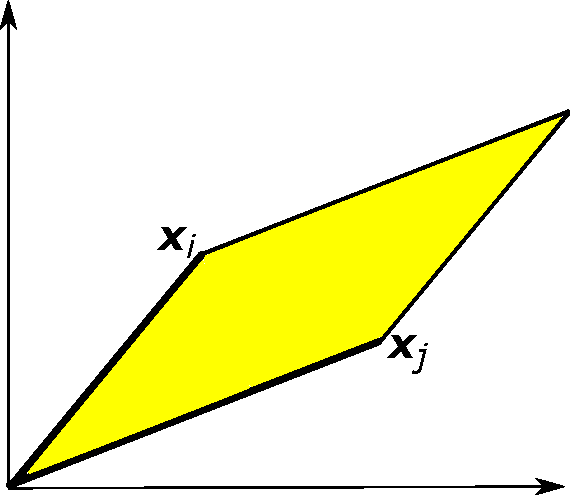
\includegraphics[width=\textwidth]{../talk/figs/volume_simple}
\end{minipage}
\vspace{7mm}

\textbf{Theorem} (from \cite{correcting-bias}) \
Volume sampling corrects the bias of any i.i.d.~sampling $q=(q_1,...,q_n)$:
\begin{align*}
\text{\footnotesize volume + i.i.d.}\quad
  &\overbrace{\x_{i_1},\,\mydots,\,\x_{i_d}}^{\sim\Vol(\X)},\
  \overbrace{\x_{i_{d+1}},\,\mydots,\,\x_{i_{k}}}^{\sim q^{k-d}}
\end{align*}
\vspace{-8mm}
\begin{align*}
  \E\bigg[\argmin_\w\sum_{t=1}^k\frac1{q_{i_t}}(\x_{i_t}^\top\w-y_{i_t})^2\bigg]
  = \w_{\y|\X}^*.
\end{align*}
    %%%%%%%%%%%%%%%%%%%%%%%%%%%%%%%%%%%%%%%%%%%%%%%%%%%%%%%%%%%%%%%%%%%%%%%%%%%%%% 
}




%%%%%%%%%%%%%%%%%%%%%%%%%%%%%%%%%%%%%%%%%%%%%%%%%%%%%%%%%%%%%%%%%%%%%%%%%%%%%%   
\headerbox{Minimax A-optimal value for experimental design}
{name=results,column=1,span=2,above=bottom,below=logloss}{
    \begin{definition}
Define the minimax A-optimal value for experimental design with
unbiased estimators as:
\begin{align*}
R_k^*(\X)&\defeq 
  \min_{(S,\wbh)\in\Wc_k(\X)}\ \max_{\y\in\Fc_n\backslash\mathrm{Sp}(\X)}\,\frac{\mathrm{MSE}\big[\wbh(\y_S)\big]-
     \mathrm{MSE}\big[\X^\dagger\y\big]
  }{\E\big[\|\xib_{\y|\X}\|^2\big]}
\end{align*}
\end{definition}
\begin{proposition} Least squares is the \textit{minimum
  variance unbiased estimator} for $\Fc_n$:
\begin{align*}
  \text{if}\quad  \E_{\y,\wbh}\big[\wbh(\y)\big]
  &=\X^\dagger\E[\y]\quad\quad\,\forall_{\y\in\Fc_n},
\\ \text{then}\quad
  \Var\big[\wbh(\y)\big]&\succeq\Var\big[\X^\dagger\y\big]\quad \forall_{\y\in\Fc_n}.
\end{align*}
\end{proposition}
\begin{theorem}
  The following statements are true about the minimax A-optimal value:
\begin{enumerate}
\item If \ $d\leq k\leq n$,\qquad\quad then \
  $R_k^*(\X)\in[0,\infty)$\quad \ for a full rank $\X$.
\item If \ $k\geq C\cdot d\log n$,\quad \,then \ $R_k^*(\X)\leq
  C\cdot\phi/k$\quad\quad\quad\!for some $C$.
  \hfill(bound from Theorem \ref{t:main})
\item If \ $k^2<\epsilon nd/3$,\qquad\ \,then \ $R_k^*(\X)\geq
  (1\!-\!\epsilon)\cdot\phi/k$\quad for some $\X$.
  \hfill(matching lower bound)
  \end{enumerate}
\end{theorem}
\renewcommand{\refname}{\normalsize References\vspace{-2mm}}
\vspace{-6mm}
{\small
  \begin{thebibliography}{3}
 \bibitem{avron-boutsidis13} H.~Avron, C.~Boutsidis. \textit{Faster subset
     selection for matrices and applications.} JMAA 2013.\vspace{-2mm}
 \bibitem{correcting-bias}M.~Derezi\'{n}ski, M.~Warmuth, D.~Hsu.
   \textit{Correcting the bias in least squares regression with
     volume-rescaled sampling.}
   AISTATS'19.
   \end{thebibliography}
}
  %%%%%%%%%%%%%%%%%%%%%%%%%%%%%%%%%%%%%%%%%%%%%%%%%%%%%%%%%%%%%%%%%%%%%%%%%%%%%% 
}


%%%%%%%%%%%%%%%%%%%%%%%%%%%%%%%%%%%%%%%%%%%%%%%%%%%%%%%%%%%%%%%%%%%%%%%%%%%%%%
\headerbox{Leverage and inverse scores}{name=entropy,column=2,below=regret,above=results}{
$\z_i$ -- $i$th column of pseudoinverse
$\underbrace{(\X^\top\X)^{-1}\X^\top}_{\X^\dagger}$
\vspace{-7mm}
  \begin{enumerate}
    \item  \textit{Leverage score sampling}: \\
      $\Pr(i)=p_i^{\mathrm{lev}}\!\defeq \frac1d
      \x_i^\top(\X^\top\X)^{-1}\x_i = \frac1d \x_i^\top\z_i$\\
{\footnotesize used to obtain a \underline{subspace embedding}}
\vspace{2mm}

\item \textit{Inverse score sampling} \Red{(new)}: \\
  $\Pr(i)= p_i^{\mathrm{inv}}\!\defeq
    \frac1\phi\x_i^\top(\X^\top\X)^{-2}\x_i = \frac1\phi \|\z_i\|^2$\\
{\footnotesize  used to get the $\phi/\epsilon$ rate for the \underline{MSE}}
  \end{enumerate}
  \vspace{2mm}
  
Controlling the least squares estimator:
  \begin{align*}
\wbh &=
    \argmin_\w\sum_{t=1}^k\frac1{q_{i_t}}(\x_{i_t}^\top\w-y_{i_t})^2\\
     &=\underbrace{\Big(\sum_{t=1}^k\frac1{q_{i_t}}\z_{i_t}\x_{i_t}^\top\Big)^{-1}}_{\text{needs
       leverage
       scores}}
       \underbrace{\sum_{t=1}^k\frac1{q_{i_t}}\z_{i_t}y_{i_t}}_{\text{needs
       inverse
       scores}}
%&=\Big(\sum_{t=1}^k\frac1{q_{i_t}}\x_{i_t}\x_{i_t}^\top\Big)^{-1}\sum_{t=1}^k\frac1{q_{i_t}}\x_{i_t}y_{i_t}
  \end{align*}
  \textbf{Strategy}: Use a mixture of both $p^{\mathrm{lev}}$ and $p^{\mathrm{inv}}$
  %%%%%%%%%%%%%%%%%%%%%%%%%%%%%%%%%%%%%%%%%%%%%%%%%%%%%%%%%%%%%%%%%%%%%%%%%%%%%% 
}


\end{poster}
  % \bibliographystyle{alpha}
  % \bibliography{../pap}


\end{document}
